% TikZ版ロードマップ図
% 統合特解理論とNKAT理論の比較研究用
\documentclass{standalone}
\usepackage{tikz}
\usetikzlibrary{positioning,arrows.meta,shapes.geometric}

\begin{document}
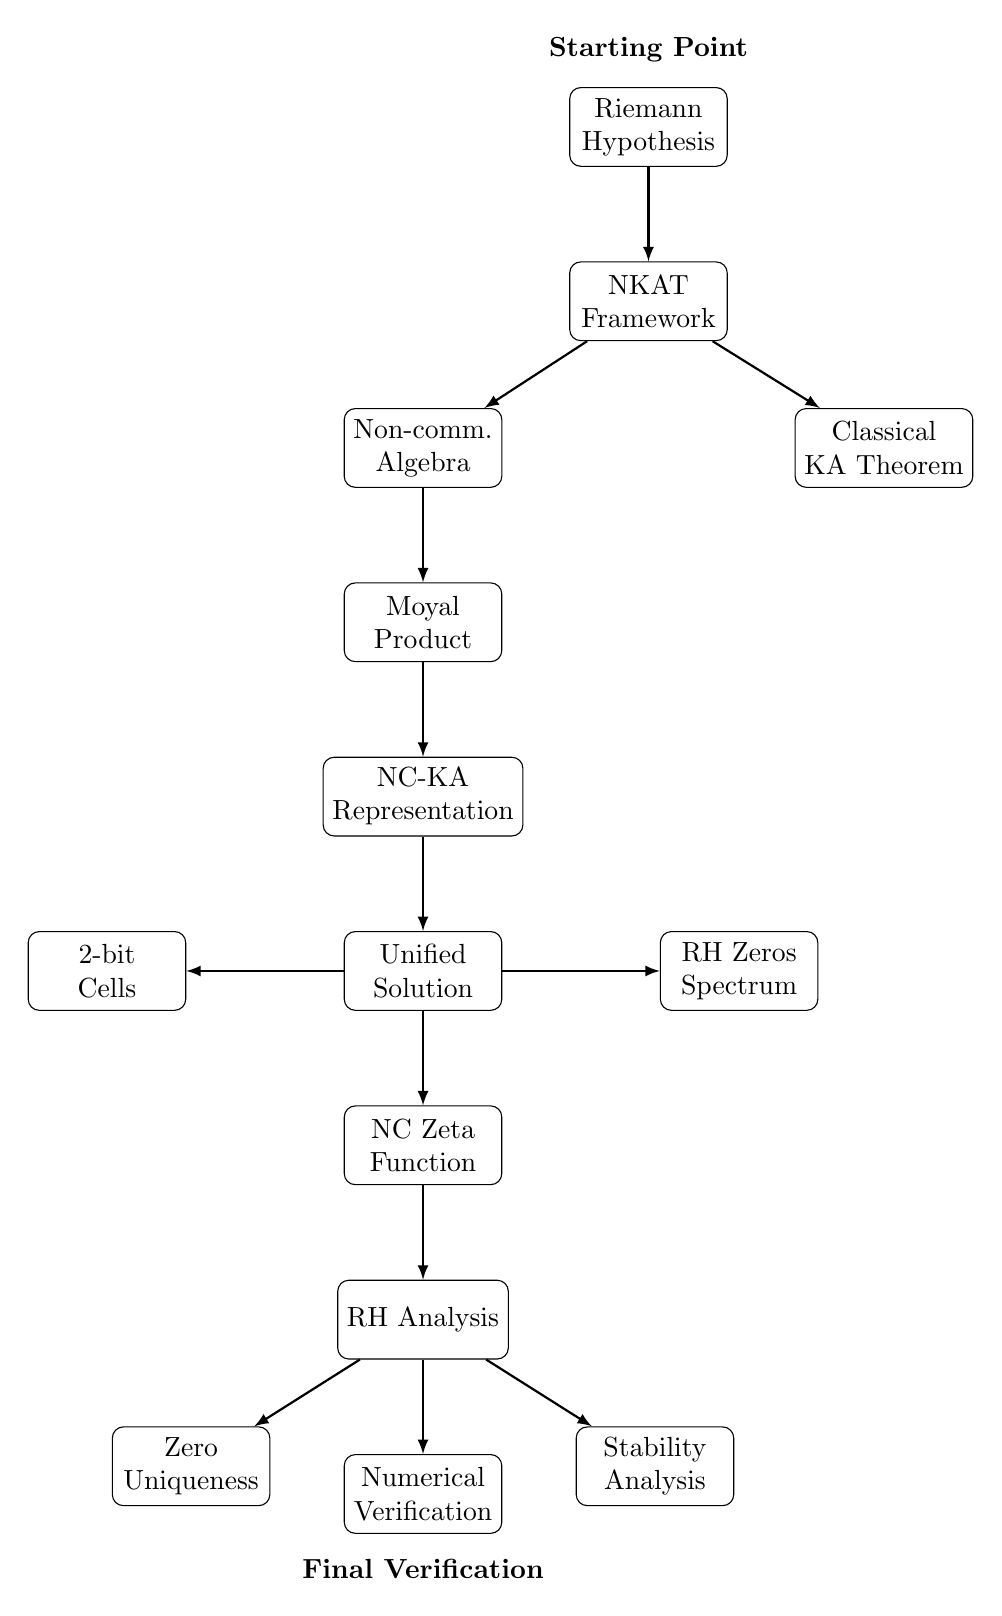
\begin{tikzpicture}[
    node distance=12mm,
    >=latex,
    block/.style={rectangle,draw,rounded corners,align=center,minimum width=2cm,minimum height=1cm},
    arrow/.style={->,thick}
]

% メインノード
\node[block] (A) {Riemann\\Hypothesis};
\node[block,below=of A] (B) {NKAT\\Framework};
\node[block,below left=of B] (C) {Non-comm.\\Algebra};
\node[block,below right=of B] (K) {Classical\\KA Theorem};
\node[block,below=of C] (D) {Moyal\\Product};
\node[block,below=of D] (E) {NC-KA\\Representation};
\node[block,below=of E] (F) {Unified\\Solution};
\node[block,left=of F,xshift=-8mm] (L) {2-bit\\Cells};
\node[block,right=of F,xshift=8mm] (M) {RH Zeros\\Spectrum};
\node[block,below=of F] (G) {NC Zeta\\Function};
\node[block,below=of G] (H) {RH Analysis};
\node[block,below left=of H] (Q) {Zero\\Uniqueness};
\node[block,below right=of H] (R) {Stability\\Analysis};
\node[block,below=of H] (I) {Numerical\\Verification};

% 矢印の描画
\draw[arrow] (A) -- (B);
\draw[arrow] (B) -- (C);
\draw[arrow] (B) -- (K);
\draw[arrow] (C) -- (D);
\draw[arrow] (D) -- (E);
\draw[arrow] (E) -- (F);
\draw[arrow] (F) -- (L);
\draw[arrow] (F) -- (M);
\draw[arrow] (F) -- (G);
\draw[arrow] (G) -- (H);
\draw[arrow] (H) -- (Q);
\draw[arrow] (H) -- (R);
\draw[arrow] (H) -- (I);

% ラベル
\node[above=2mm of A] {\textbf{Starting Point}};
\node[below=2mm of I] {\textbf{Final Verification}};

\end{tikzpicture}
\end{document} 